\documentclass[conference]{IEEEtran}
\IEEEoverridecommandlockouts
% The preceding line is only needed to identify funding in the first footnote. If that is unneeded, please comment it out.
\usepackage{cite}
\usepackage{amsmath,amssymb,amsfonts}
\usepackage{algorithmic}
\usepackage{graphicx}
\usepackage{textcomp}
\usepackage{xcolor}
\usepackage{float}
\usepackage{caption}
\usepackage{booktabs}
\usepackage{url}
\def\BibTeX{{\rm B\kern-.05em{\sc i\kern-.025em b}\kern-.08em
    T\kern-.1667em\lower.7ex\hbox{E}\kern-.125emX}}

%\addbibresource{../book/misc/bibliography.bib}


\begin{document}

\title{YOLOv911: An Improvement to YOLOv7 for Airborne Object Detection Task\\ 
%{\footnotesize \textsuperscript{*}Note: Sub-titles are not captured in Xplore and
%should not be used}
%\thanks{Identify applicable funding agency here. If none, delete this.}
}

\author{
    Dion Andreas Solang, Reza Fuad Rachmadi, I Ketut Eddy Purnama\\
    Department of Computer Engineering\\
    Faculty of Intelligent Electrical and Information Technology\\
    Institut Teknologi Sepuluh Nopember (ITS)\\
}


%\author{\IEEEauthorblockN{1\textsuperscript{st} Given Name Surname}
%\IEEEauthorblockA{\textit{dept. name of organization (of Aff.)} \\
%\textit{name of organization (of Aff.)}\\
%City, Country \\
%email address or ORCID}
%\and
%\IEEEauthorblockN{2\textsuperscript{nd} Given Name Surname}
%\IEEEauthorblockA{\textit{dept. name of organization (of Aff.)} \\
%\textit{name of organization (of Aff.)}\\
%City, Country \\
%email address or ORCID}
%\and
%\IEEEauthorblockN{3\textsuperscript{rd} Given Name Surname}
%\IEEEauthorblockA{\textit{dept. name of organization (of Aff.)} \\
%\textit{name of organization (of Aff.)}\\
%City, Country \\
%email address or ORCID}
%\and
%\IEEEauthorblockN{4\textsuperscript{th} Given Name Surname}
%\IEEEauthorblockA{\textit{dept. name of organization (of Aff.)} \\
%\textit{name of organization (of Aff.)}\\
%City, Country \\
%email address or ORCID}
%\and
%\IEEEauthorblockN{5\textsuperscript{th} Given Name Surname}
%\IEEEauthorblockA{\textit{dept. name of organization (of Aff.)} \\
%\textit{name of organization (of Aff.)}\\
%City, Country \\
%email address or ORCID}
%\and
%\IEEEauthorblockN{6\textsuperscript{th} Given Name Surname}
%\IEEEauthorblockA{\textit{dept. name of organization (of Aff.)} \\
%\textit{name of organization (of Aff.)}\\
%City, Country \\
%email address or ORCID}
%}

\maketitle

\begin{abstract}    
In this research, we present some approach to improve the capability of YOLOv7
to detect airborne objects. Airborne objects appear very small on cameras due
to their usually large distance to the camera. For that reason, YOLOv7 needs to
be optimized to detect small objects. Several modification proposals was made and
tested in this research. The modifications include changes in the architecture
(adding extra detection layer, modifying feature-map source of the neck,
and replacing detection head to a detached anchor-free head) and in Bag-of-Freebies
(anchor recalculation and mosaic augmentation). We found the combination of
mosaic augmentation, anchor recalculation, and modification of feature-map source of
the neck produces a model with mAP 14.09\%, a significant improvement compared
to plain YOLOv7 that produces mAP of 0\%.
%This document is a model and instructions for \LaTeX.
%This and the IEEEtran.cls file define the components of your paper [title, text, heads, etc.]. *CRITICAL: Do Not Use Symbols, Special Characters, Footnotes, 
%or Math in Paper Title or Abstract.

\end{abstract}

\begin{IEEEkeywords}
Small Object Detection, YOLOv7, Architecture Modification, Bag-of-Freebies Modification, Airborne Object
\end{IEEEkeywords}

\section{Introduction}

Autonomous Aerial Vehicle (AAV) has been gaining a lot of popularity lately.
As said on \cite{prime_air}, AAV are now being developed for commercial use.
This brings challenges for the AAV as it would need to have a good Sense and Avoid (SAA)
ability. 

As most drone uses camera as its sensor due to its smaller weight and lower price, 
there is a need for camera based object detection system for SAA purpose.
One problem is that, airborne objects appear very small on the camera due 
to their distance to the camera (but they approach the camera very fast). Thus,
the object detection system must be able to detect small objects.

In this research, we attempt to optimize YOLOv7 to be able to perform airborne
object detection. YOLOv7 was chosen due to its ability to perform real-time
object detection accurately. YOLOv7 had the highest mAP score amongst all
published real-time object detector at the time of the execution of this research \cite{yolov7}.

To optimize YOLOv7, we defined a set of modification to be applied to YOLOv7
that includes modification to its neural network architecture and some applications
of bag-of-freebies. To find to optimal solution, we will try combinations of
the modification within the set, and choose the one with the highest mAP score.

We will be using The Airborne Object Tracking (AOT) Dataset \cite{aot_dataset} to train
and test the modification combinations. AOT Dataset consist of aerial vehicle flights
footage. In this dataset, the resolution of each image are $2048\times2448$ px, meanwhile
the size of the airborne object bounding box can be as small as 4 px (0.00008\% of resolution).
You can see an example of the dataset in Fig. \ref{fig:airborne-example}.
\begin{figure}[htbp]
\centerline{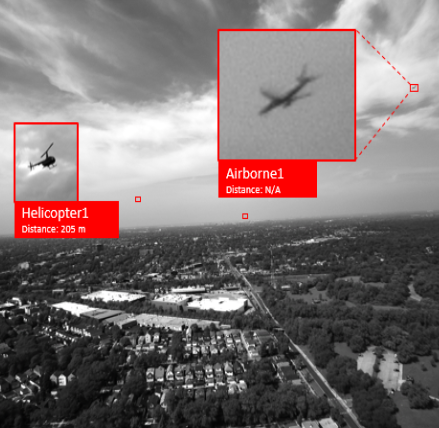
\includegraphics[width=0.4\textwidth]{../book/figures/dataset-example-labeled.png}}
\caption{Example Image from AOT Dataset \cite{aot_docs}}
\label{fig:airborne-example}
\end{figure}

\section{Related Works}
Several attempts have been made in the past to increase YOLO architecture ability
to detect small objects. Here we present some of them.
\subsection{YOLO-Z}
YOLO-Z is a modification of YOLOv5 to optimize its ability to detect
cone for autonomous racing purpose \cite{yoloz}.
YOLO-Z modify the backbone of YOLOv5r5.0 to down-scaled DenseNet, while
the neck was changed to PanNet.
These modification results in an increase of accuracy to detect cone
that are far away while still being able to do detection in real-time.
\subsection{exYOLO}
exYOLO bases its modification on YOLOv3 \cite{exyolo}. exYOLO modifies
the neck by adding Receptive Field Block before combining the feature maps.
These modifications produce a higher mAP score than plain YOLOv3 on
PASCAL VOC2007 dataset.

\section{Experimental Setup}

\subsection{Instruments}
\label{section:instruments}
To conduct the experiment, we use Nvidia RTX 2080 Ti GPU which has 11 GB of VRAM.
In this limited amount of memory, training large YOLOv7 model such as W6, E6, and E2E
become infeasible. Not to add the large input size of the image. For this reason,
the architecture that is chosen as the baseline for modification is the normal  size
YOLOv7. The model will be trained with input size of $1600\times1600$ with batch size 1.

Furthermore, the dataset that will be used to train the model will be limited to 400 images.
The sampling strategy for the dataset will be explained in section \ref{section:dataset}.
In a pilot test of the experiment, we found that to train a model for 300 epochs with 400 images
with this setup, it will take around 20 hours. This is the reason why we limit the 
amount of images to 400 and epoch to 300.

\subsection{Dataset}
\label{section:dataset}
The AOT dataset, consist of more than 11 TB images of drone camera footage.
Amongst these 11 TB of data, there are images taken from planned and unplanned encounters with
airborne objects. In this research, we sample the data from planned encounters.
There are millions of image in the planned encounters. To obtain 400 images
for training as explained in section \ref{section:instruments}
and some more for validation and testing, we use the sampling strategy
described in Table \ref{tbl:datasetsamplingdist}.

\begin{table}[htbp]
  \centering
  \caption{Dataset Sampling Strategy}
  \label{tbl:datasetsamplingdist}
  %\resizebox{\columnwidth}{!}{%
  \tabcolsep4pt
  \begin{tabular}{c c c c c c c}
    \toprule[1.5pt]
              &Total & \multicolumn{5}{c}{Percentage}\\
%                       \cline{3-7}
              &Images&Airplane & Helicopter & Bird & Drone & Negative\\
    \midrule
    Training  &400 &23.75\%    &23.75\%     &23.75\% &23.75\%       &5\%\\
    \midrule
    Validation&100  &20\%      &20\%        &20\%    &20\%          &20\%\\
    \midrule
    Test      &200  &20\%      &20\%        &20\%    &20\%          &20\%\\
    \bottomrule[1.5pt]
  \end{tabular}%
  %}
\end{table}


\subsection{Modifications}
\label{section:modifications}
We proposed some modifications that can be applied to YOLOv7

\subsubsection{Mosaic Augmentation}
Mosaic Augmentation was reported to increase the mAP score of the model in
\cite{yolov4}{yolov5}. This augmentation is simple to implement. Therefore,
we included mosaic augmentation in our set of modifications combine.

\subsubsection{Anchor Recalculation}
Anchor points that were available on the implementation code of YOLOv7
are optimized for COCO2017 dataset. As the AOT dataset distribution
are heavily skewed, the anchors need to be adjusted to match the data distribution.
For this reason, anchor recalculation is included in our set of modifications.

\subsubsection{EIoU localization loss}
The localization loss used in YOLOv7 is CIoU.
Both EIoU and CIoU are designed to solve the vanishing gradient problem of the standard
IoU. The advantage EIoU has over CIoU is that when the bounding boxes intersect, EIoU
behaves like the standard IoU while CIoU doesn't. The metrics used to evaluate the models
like mAP are based on the standard IoU, thus it's better for the loss function to mimic the metric \cite{eiou}.
\cite{eiou} reported that EIoU performs better on Faster-RCNN than CIoU, making this modification
a good candidate to be tested on YOLOv7.

\subsubsection{Modify Neck Feature-map Source}
\begin{figure}[htbp]
\centerline{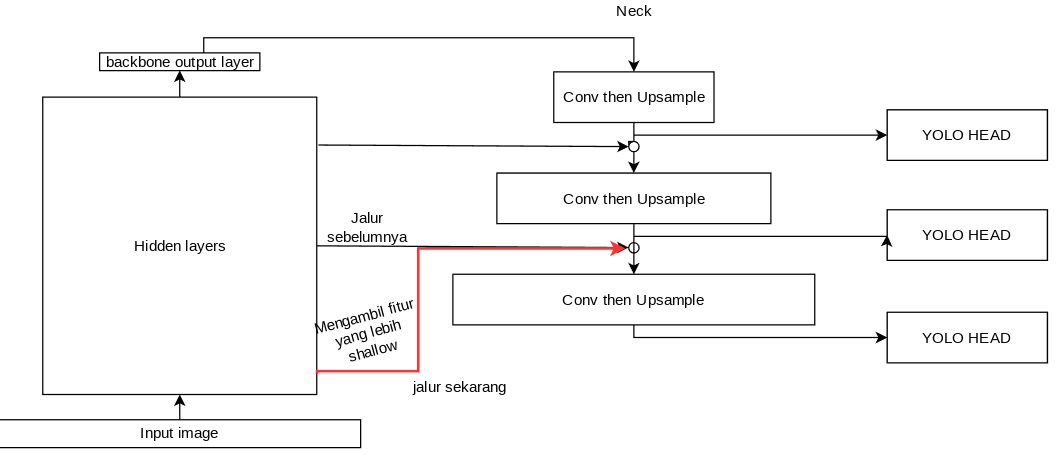
\includegraphics[width=0.4\textwidth]{../book/figures/neck-move-back.png}}
\caption{Moving Neck Feature-map Source}
\label{fig:neck-move-back}
\end{figure}
The source feature map that was fed on the feature pyramid can be moved
to a shallower layer of the backbone (look at Fig. \ref{fig:neck-move-back}). 
The shallower layer (layers that are closer to the input) has more 
information about the image, albeit have less abstraction. 
By doing this, we avoid the loss of information.

\subsubsection{Additional Detection Layer}
\begin{figure}[htbp]
\centerline{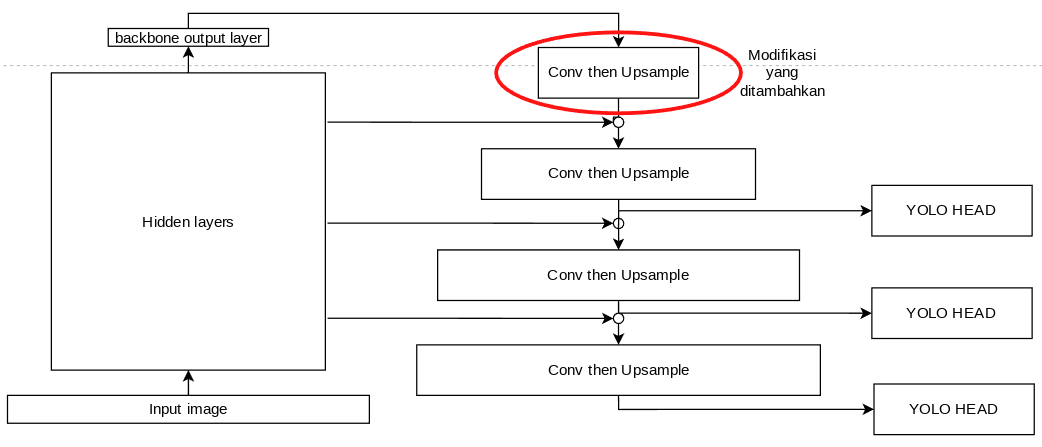
\includegraphics[width=0.4\textwidth]{../book/figures/add-more-upsampling.png}}
\caption{Adding More Detection Layer}
\label{fig:add-head}
\end{figure}
An additional detection layer enable YOLOv7 to detect at more scales. With more scales,
the detection layers can be more specialized to specific cluster of data.
This approach has been tried in \cite{barunastra} by increasing the number of
detection layer from 2 to 3 in YOLOv4-tiny. In this experiment, we will increase
the number of detection layer from 3 to 4.
\subsubsection{Replacing Detection Layer to Decoupled Anchor-Free Head}
One of the advantage of anchor-free model to anchor-based model
is that it decreases the amount of heuristic tuning parameter as we don't
have to define the anchors. \cite{yolox} reported that using anchor-free
head increases the accuracy and decreases the number of parameters in the model,
resulting in a faster and more accurate model.

\section{Result}
\subsection{Initial Performance}
At first, we evaluate the performance of a plain YOLOv7 without all the
modifications proposed in section \ref{section:modifications}.
With 300 epochs and 400 data sample, we find the model was unable to detect
anything in the test set (mAP = 0).
For the purpose of comparison with other modification combination,
we will call this model as \verb*|YOLOv7-plain|.

\begin{figure*}
\centerline{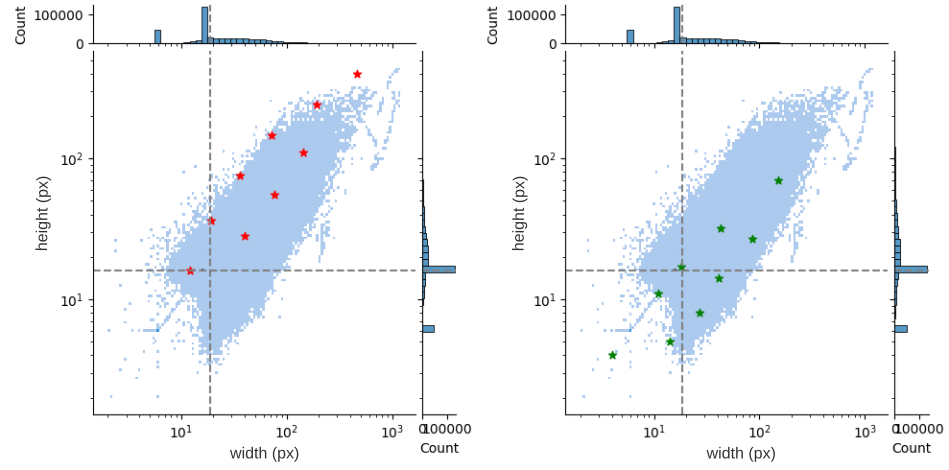
\includegraphics[width=0.9\textwidth]{../book/figures/anchor-dist-2.png}}
\caption{Anchor Points in Dataset Distribution. Left: Original Anchors. Right: Recalculated Anchors}
\label{fig:anchor-recalculated}
\end{figure*}

\subsection{Mosaic Augmentation and Anchor Recalculation}
In this section, we will compare 3 modification combination
\begin{itemize}
    \item YOLOv7-plain + Mosaic
    \item YOLOv7-plain + Anchor Recalculation
    \item YOLOv7-plain + Mosaic + Anchor Recalculation
\end{itemize}
We calculated the anchors using k-means clustering algorithm on the
training dataset. The result of the recalculation can be seen on Fig. \ref{fig:anchor-recalculated}.
As can be seen on the figure, 8 out of 9 of the old anchor points are placed in the first quadrant
of the median line. This means that those 8 anchors responsible only for 25\% of the dataset, which
is very ineffective. Compare that to the recalculated anchor. Every quadrant has at least one anchor
point responsible to it.
\begin{table}[htbp]
  \centering
  \caption{Mosaic Augmentation and Anchor Recalculation Performance}
  \label{tbl:mosaic_reanchor_performance}
  \vspace{-1ex}
  \begin{tabular}{ l l c }
    \toprule[1.5pt]
    No & Modification        &mAP@50 \\
    \midrule
    0  & \textbf{YOLOv7-plain               }& 0\%\\
    1  & \textbf{YOLOv7-plain + mosaic                     }& 0\%\\
    2  & \textbf{YOLOv7-plain + anchor recalculation         }& 0\%\\
    3  & \textbf{YOLOv7-plain + mosaic + anchor recalculation}& \textbf{11,2}\%\\
    \midrule
       & Improvement                         & \textbf{\textcolor{green}{+11,2\%}}\\
    \bottomrule[1.5pt]
  \end{tabular}
\end{table}
Table \ref{tbl:mosaic_reanchor_performance} shows that the model was only able
to detect something on the test dataset after being applied mosaic augmentation
and anchor recalculation.

This model will be used as the basis for further 
modification, as it was the only model that could detect objects in test dataset.
For this reason, this combination of modification shall be called \verb*|YOLOv7-base|
from this point on.

\subsection{EIoU Localization Loss}
In addition to just using EIoU, we also tested EIoU with its convexication technique 
mentioned in \cite{eiou}. The result can be seen on Table \ref{tbl:loss_function_perf}
\begin{table}[htbp]
  \centering
  \captionof{table}{EIoU Localization Loss Performance}
  \label{tbl:loss_function_perf}
  \vspace{-1ex}
  \begin{tabular}{ l l c }
    \toprule[1.5pt]
    No & Modifikasi        &mAP@50 \\
    \midrule
    0  & \textbf{yolov7-base + CIoU (original)}     & \textbf{11,2}\%\\
    1  & \textbf{yolov7-base + EIoU}                & 0\%\\
    2  & \textbf{yolov7-base + EIoU + Convexication} & 4.92\%\\
    \midrule
       & Improvement                                & \textbf{\textcolor{red}{-6.28\%}}\\
    \bottomrule[1.5pt]
  \end{tabular}
\end{table}
It turns out that EIoU only worsen the performance of YOLOv7 in AOT dataset.

\subsection{Modify Neck Feature-map Source}
\begin{figure}[htbp]
\centerline{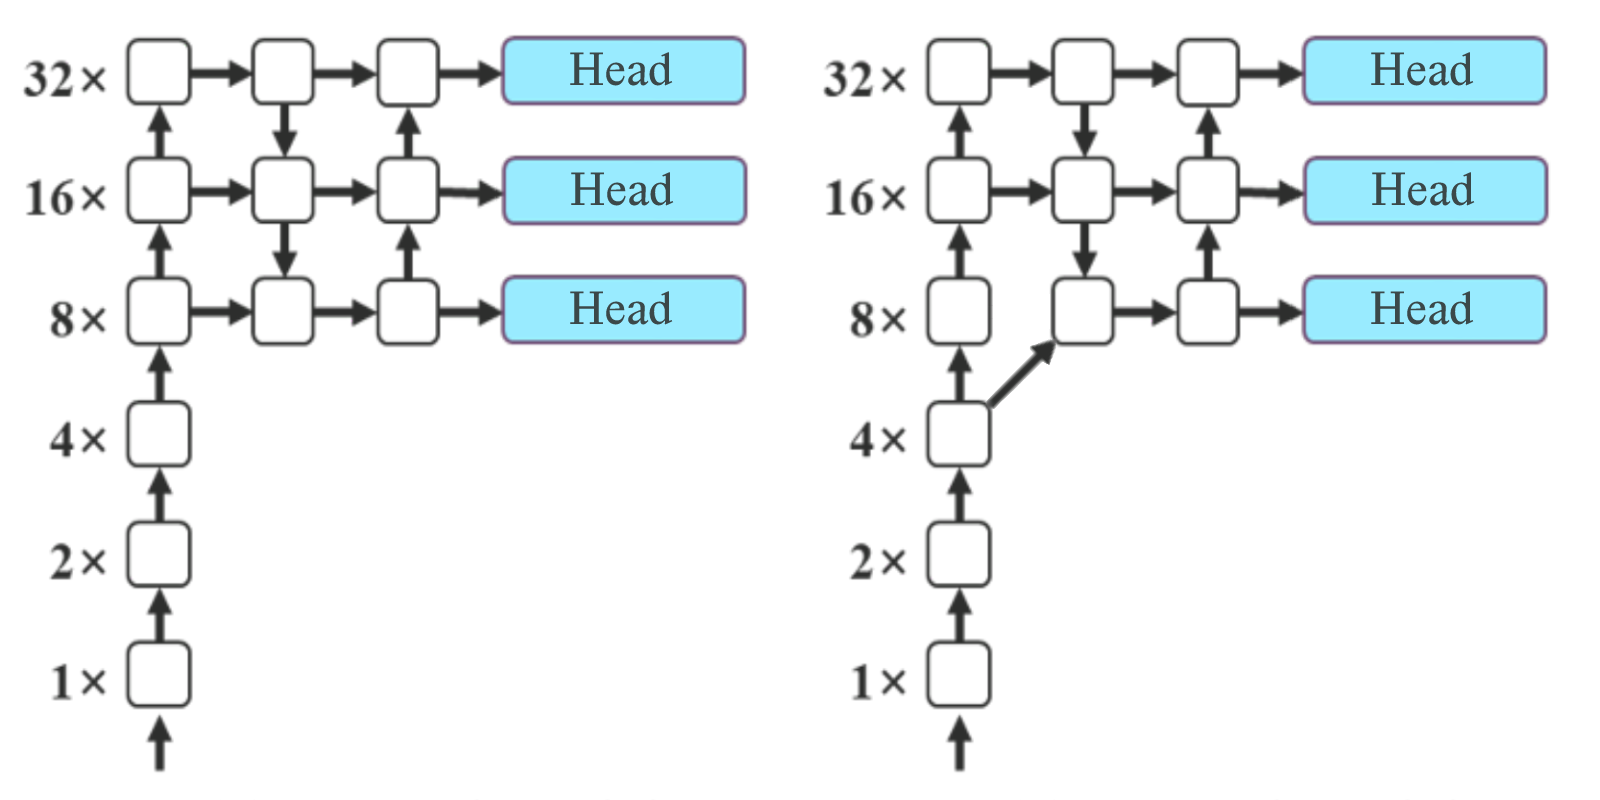
\includegraphics[width=0.5\textwidth]{../book/figures/deeperconn.png}}
\caption{Moving Feature-map Source}
\label{fig:deeperconn}
\end{figure}
We move the connection of the first pyramid from scale 8 to scale 4 of the backbone.
That is from layer 24 to layer 11 of the configuration file.
The moving of this connection is illustrated in Fig. \ref{fig:deeperconn}.
The performance of this modification can be seen on Table \ref{tbl:neck_backbone_perf}.
\begin{table}[htbp]
  \centering
  \caption{Moving Feature-map Source Performance}
  \label{tbl:neck_backbone_perf}
  \vspace{-1ex}
  \begin{tabular}{ l l c }
    \toprule[1.5pt]
    No & Modification                                      &mAP@50 \\
    \midrule
    0  & \textbf{yolov7-base}                            & 11.2\%\\
    1  & \textbf{yolov7-base + modifikasi neck-backbone} & \textbf{14.09\%}\\
    \midrule
       & Improvement                                & \textbf{\textcolor{green}{+2.98\%}}\\
    \bottomrule[1.5pt]
  \end{tabular}
\end{table}
This modification managed to increase the mAP score by 2.98\%.
For the purpose of comparison with other modification combinations, we shall call
this model \verb*|YOLOv7-moveconnection| from this point on.


\subsection{Adding Extra Detection Layer}
\begin{figure}[htbp]
\centerline{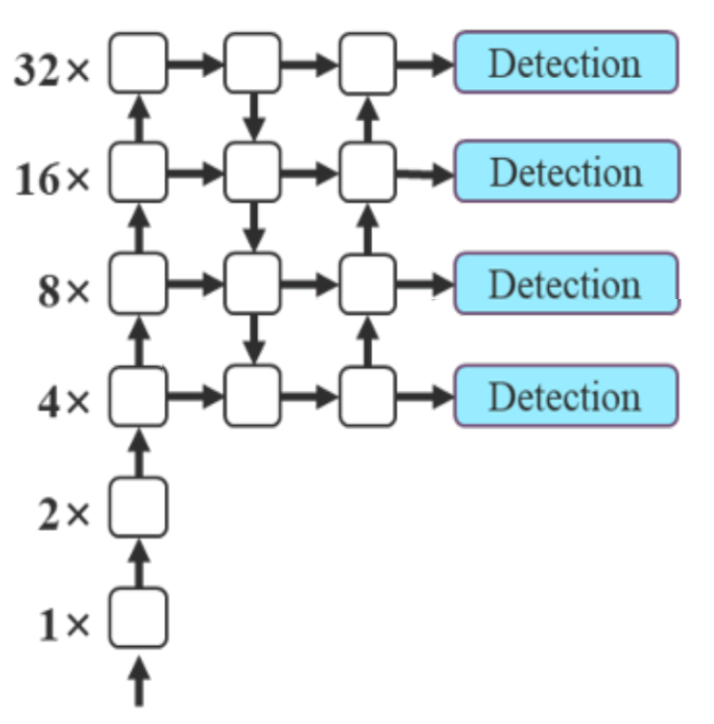
\includegraphics[width=0.4\textwidth]{../book/figures/addhead.png}}
\caption{Adding More Detection Layer}
\label{fig:add-head-2}
\end{figure}
We add an extra feature pyramid stage connected to scale 4 of the backend, and put a detection head on it.
This modification is illustrated in Fig. \ref{fig:add-head-2}. We find that this modification
perform worse than YOLOv7-moveconnection as seen on Table \ref{tbl:addhead}.
\begin{table}[htbp]
  \centering
  \captionof{table}{Performance of Adding Extra Detection Layer}
  \label{tbl:addhead}
  \vspace{-1ex}
  \begin{tabular}{ l l c }
    \toprule[1.5pt]
    No & Modifikasi                                 &mAP@50 \\
    \midrule
    0  & \textbf{yolov7-base}                       & \textbf{11.2\%}\\
    1  & \textbf{yolov7-base + additional head}       & 5.19\%\\
    \midrule
       & Improvement                                & \textbf{\textcolor{red}{-6\%}}\\
    \bottomrule[1.5pt]
  \end{tabular}
\end{table}

\subsection{Decoupled Anchor-free Head}
We changed the head of the model to anchor-free head with Task Aligned Labelling.
It resulted in 0 mAP.


\section{Conclusion}
From the result of the experiment, we can conclude that, from the set of modification
candidates proposed in this research, we found that the combination of mosaic augmentation,
anchor recalculation, and modifying the connection of neck and backbone produces a model
with the greatest mAP score which is 14.09\%.

\section{Discussion}
As of today, the modification proposed in this research only includes the modification that
doesn't significantly impact the latency of the model. Some modification like partitioning
the image and perform detection on each of partition could produce a great increase in mAP
as the objects are magnified (number of partition) times. The latency also multiplied
by the number of partition. But we can make the model faster by down-scaling the model.
Thus, it is needed to find the optimal combination between down-scaling and number of partition
that can produce a model that have high accuracy, but still have a latency that can be categorized
as real-time.



%\begin{table}[htbp]
%\caption{Table Type Styles}
%\begin{center}
%\begin{tabular}{|c|c|c|c|}
%\hline
%\textbf{Table}&\multicolumn{3}{|c|}{\textbf{Table Column Head}} \\
%\cline{2-4} 
%\textbf{Head} & \textbf{\textit{Table column subhead}}& \textbf{\textit{Subhead}}& \textbf{\textit{Subhead}} \\
%\hline
%copy& More table copy$^{\mathrm{a}}$& &  \\
%\hline
%\multicolumn{4}{l}{$^{\mathrm{a}}$Sample of a Table footnote.}
%\end{tabular}
%\label{tab1}
%\end{center}
%\end{table}

%\begin{figure}[htbp]
%\centerline{\includegraphics{fig1.png}}
%\caption{Example of a figure caption.}
%\label{fig}
%\end{figure}

%Figure Labels: Use 8 point Times New Roman for Figure labels. Use words 
%rather than symbols or abbreviations when writing Figure axis labels to 
%avoid confusing the reader. As an example, write the quantity 
%``Magnetization'', or ``Magnetization, M'', not just ``M''. If including 
%units in the label, present them within parentheses. Do not label axes only 
%with units. In the example, write ``Magnetization (A/m)'' or ``Magnetization 
%\{A[m(1)]\}'', not just ``A/m''. Do not label axes with a ratio of 
%quantities and units. For example, write ``Temperature (K)'', not 
%``Temperature/K''.

%\section*{Acknowledgment}
%
%The preferred spelling of the word ``acknowledgment'' in America is without 
%an ``e'' after the ``g''. Avoid the stilted expression ``one of us (R. B. 
%G.) thanks $\ldots$''. Instead, try ``R. B. G. thanks$\ldots$''. Put sponsor 
%acknowledgments in the unnumbered footnote on the first page.

%\section*{References}

\bibliographystyle{IEEEtran}
\bibliography{../book/misc/bibliography}

%\begin{thebibliography}{00}
%\bibitem{b1} G. Eason, B. Noble, and I. N. Sneddon, ``On certain integrals of Lipschitz-Hankel type involving products of Bessel functions,'' Phil. Trans. Roy. Soc. London, vol. A247, pp. 529--551, April 1955.
%\bibitem{b2} J. Clerk Maxwell, A Treatise on Electricity and Magnetism, 3rd ed., vol. 2. Oxford: Clarendon, 1892, pp.68--73.
%\bibitem{b3} I. S. Jacobs and C. P. Bean, ``Fine particles, thin films and exchange anisotropy,'' in Magnetism, vol. III, G. T. Rado and H. Suhl, Eds. New York: Academic, 1963, pp. 271--350.
%\bibitem{b4} K. Elissa, ``Title of paper if known,'' unpublished.
%\bibitem{b5} R. Nicole, ``Title of paper with only first word capitalized,'' J. Name Stand. Abbrev., in press.
%\bibitem{b6} Y. Yorozu, M. Hirano, K. Oka, and Y. Tagawa, ``Electron spectroscopy studies on magneto-optical media and plastic substrate interface,'' IEEE Transl. J. Magn. Japan, vol. 2, pp. 740--741, August 1987 [Digests 9th Annual Conf. Magnetics Japan, p. 301, 1982].
%\bibitem{b7} M. Young, The Technical Writer's Handbook. Mill Valley, CA: University Science, 1989.
%\end{thebibliography}
%\vspace{12pt}
%\color{red}
%IEEE conference templates contain guidance text for composing and formatting conference papers. Please ensure that all template text is removed from your conference paper prior to submission to the conference. Failure to remove the template text from your paper may result in your paper not being published.

\end{document}
